\pattern{Decorator}
\begin{summary}
    Decorator pattern allows functionalities to be added or removed from an
    existing object, either statically or dynamically, without changing its
    original structure. Also, in these processes, the behavior of other objects
    from the same class will not be influenced. It resolves the problem when
    subclassing would result a large number of subclasses. It is also known
    as ``Wrapper'' Pattern because this pattern utilized a ``wrapper'' (decorator class)
    that wraps the original object and appends more functionalities while leaving
    class methods signature unchanged.
\end{summary}

\subsubsection{Implementation}
Composite and Decorator have similar structure diagrams since they both rely on
recursive composition to organize a number of objects. Comparing with composite
pattern, the decorator pattern can be viewed as a degenerate composite with
only one component. However, a decorator adds additional responsibilities.

Component: It is an interface implemented by both, concrete component and
decorators. It is also the interface for objects that can have functionalities
added to them dynamically.

Concrete Component: Normally, it is known as a base which needs to be
decorated. It also defines an object to which additional functionalities can be
added or removed.

Decorator: It represents a base class for all decorators. It maintains a
reference to a component object and defines an interface that conforms to
component interface.

Concrete Decorator (ie. Co ncreteDecA, ConcreteDecB): It extends the
functionality of the component by adding state or adding behavior.

\comparison{\begin{itemize}
        \item Decorator Pattern is flexible and easy to extend functionalities.
        \item Decorator Pattern is a good solution to permutation issues
            because a concrete pattern can be wrapped with any number of
            decorators.
        \item Decorators allow behavior modification at runtime rather than
            going back into existing code and making changes.
        \item It is easy to debug each functionality seperately.

    \end{itemize}

}{\begin{itemize}
        \item Since there are many decorators warp around the component, it is
            hard to have decorators keep track of other decorators.
        \item It can be complicated to initialize a concrete component wrapped
            with many decorators. Sometimes, we may miss some of them.
        \item Abstract decorator must provide common interface.
    \end{itemize}
}%END comparison

\begin{nfps}
\item[Complexity] The pattern is extremely reusable by adding new object types
    in the decorator section to fit in what system requires and needs. New object
    types can be built on objects that already exist. It is easy for them to
    decorate these objects because decorator pattern is efficient and flexible.
\end{nfps}

\begin{center}
    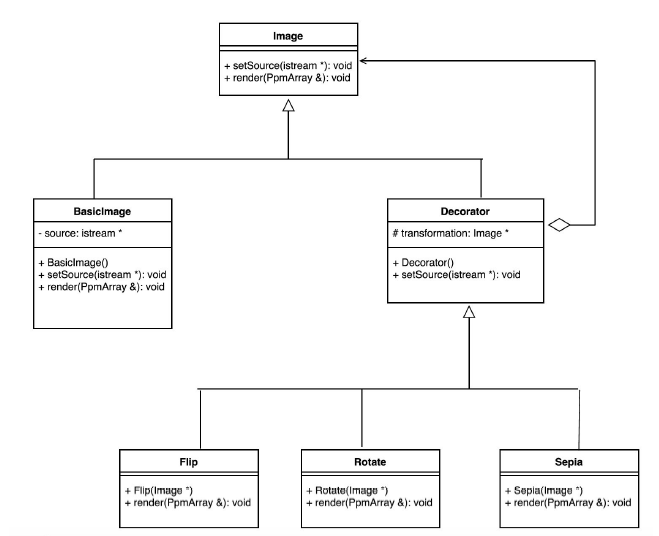
\includegraphics[width=0.8\textwidth]{./decorator}
\end{center}
